\chapter{CellTAN: Cellular Time Activation Networks} \label{chap:chap4}

Distributed information systems characterized by time series data present various challenges, primarily due to their complex and dynamic nature. The sheer volume of data that must be processed and analyzed in real time is a significant challenge, leading to concerns over storage, computation, and scalability. Moreover, data quality issues such as missing or incomplete data and data heterogeneity arising from sourcing data from disparate sources with varying consistency and structure further exacerbate these challenges. Another critical challenge of these systems is handling the temporal aspects of time series data, requiring specialized pre-processing, feature extraction, and modeling techniques. The distributed nature of these systems further complexifies matters, with issues encompassing data synchronization and accuracy being a common concern. Furthermore, their implementation in real-world applications requires robust mechanisms for data security and privacy, which adds a layer of complexity to the design and implementation of these systems.

\begin{figure}[h!]
    \centering
    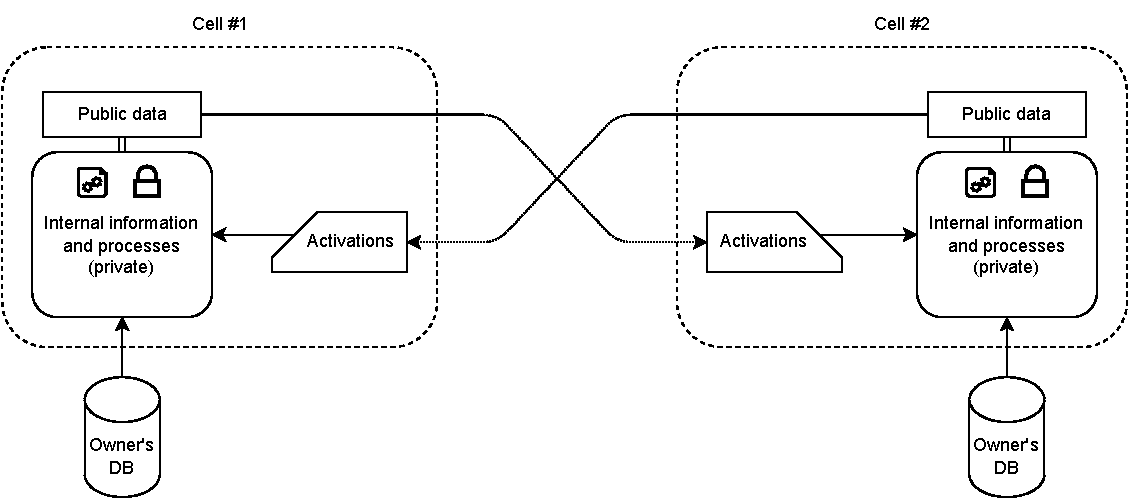
\includegraphics[width=12cm]{figures/chapter4/cell/intro.pdf}
    \caption{Simples CellTAN Network of two cells cooperating.}
    \label{fig:celltanintro}
\end{figure}

This chapter proposes a novel tool entitled CellTAN (Cellular Time Activation Network) that undertakes those challenges. CellTAN represents sparse yet interconnected components that function independently, cooperatively, and asynchronously. Inspired by other effective mechanisms like GNNs, CXNs, and Weighted Cross-Connection Networks (WCCNs), CellTAN uses a graph-like structure to represent a network of components, with nodes and connections. Following the introductory chapters, its primary purpose is to detect anomalous scenarios on PV systems. However, its generalized formulation introduces other valuable features which come naturally from fulfilling this goal. Such are state estimation, forecasting, and capturing the value in data from different PV asset owners without violating their privacy. For briefness' sake, we will the details about its benefits to be unfolded during the rest of this chapter.

Instead of tackling fault detection and classification in a classical centralized manner, which is already extensively showcased throughout the literature, this tool approaches this problem with a paradigm change: a distributed and asynchronous data coherence system. By having a virtual representation closely related to the physical form of sparse systems, relationships between components can be leveraged to assess their correct (or incorrect) operation. While initially designed for photovoltaic (PV) systems, the concepts of cells, connections, neighbors, time series, and uncertainty are universal and applicable to other fields such as biology, physics, and more. Thus, the potential for generic applicability sparks the interest to not bake specifics of PV systems directly into this tool, allowing its usage for other subjects. Figure \ref{fig:celltanintro} represents minimal scenario for a network: only two cells. It showcases some terms specific to this tool, that might be difficult to grasp at first, such as trust, events, and activations. Consequently, the glossary in \ref{sec:glossary} and detailed explanations throughout this chapter serve to clarify them.

Vast and scattered information across multiple agents is a common scenario faced by the industry of AI for energy systems, which cannot be aggregated due to privacy and confidentiality reasons. Nevertheless, its conjunction could have a lot of added value, given the similarity of certain assets: PV plants (as well as wind farms) from different owners in neighbouring geographical regions. This information-sharing potential for AI algorithms motivates the development of a mechanism that provides a way of communicating information between differently owned assets without any of the compromises above. However, and as stated before, data acquisition in PV scenario's is scarcely synchronous and might not occur in equal time resolutions for all the different components. The CellTAN addresses these issues with an instrument referred to as \textbf{Time activations}. It proposes a new way of communication that decouples from the needs of units, sampling rate, and synchronization, avoiding any resampling, normalization, or even obfuscation (to protect privacy). This mechanism is a core feature of the tool since it will be the means that will allow connecting different stakeholders' data, hence section \ref{sec:thecell} develops this matter thoroughly. Likewise, succeeding sections formulate the working of the \textbf{Cell} and its interactions within the network. Since it is the core component, understanding its behavior is crucial for a complete understanding of the tool.

\section{Glossary} \label{sec:glossary}


\begin{itemize}
    \item \textbf{Knowledge base}: Refers to registered historical knowledge (samples) of time series variables.
    
    \item \textbf{Inputs}: Uniform fuzzy numbers (not necessarily, but it's the current choice) that represent one sample of the group of time series variables that define the state of a cell.

    \item \textbf{Outputs}: Similar to inputs, but obtained through mroe complex computations.

    \item \textbf{Time decay}: A process associated with increased uncertainty of variables over time.
    
    \item \textbf{Activations}: Timestamps of past ocurrences on a knowledge base that have a non zero value of membership against a set of recent inputs.
    
    \item \textbf{Events}: Occurences that the cell reports back to the hub, that in most cases are triggered by the exceeding of parametrized thresholds.
    
    \item \textbf{Trust}: A decimal number that represents how coherent two cells's activations are with each other. Besides its instantaneous computed value, it can also come from a cumulative computation on a defined time window.

    \item \textbf{Hub}: The central component of the cell network, which facilitates its visualization, management, and expansion. It acts as the proxy agent between the cell's communication.
    
\end{itemize}

\section{The Cell} \label{sec:thecell}

A cell is an independent entity composed of \textbf{data} and \textbf{processes}. The main idea is to abstract fundamental system components (e.g. inverters, MPPT's) into this virtual entity. With an added layer of intelligence, it will assess their current state, adding value to the existing data acquisition and monitoring systems.
For this, it features an intrinsic inference algorithm that takes advantage of uncertainty in the input variables to . 

% TODO maioria da descrição fazê-la aqui

As an individual part of the system, it follows a set of rules that define its intrinsic and extrinsic behavior. These rules address data privacy, request boundaries, and real-world operational limitations.

\paragraph*{Independence} During operation, independence on neighbors or other network entities for continuous processing of outputs results in a more robust system and increases availability. Thus, given any connection cutoffs, the cell shall be unbothered by its surroundings and continue operating in an isolated state. Isolation is not preferred, but enduring it until outside contact is re-established avoids shutdown and startup procedures. 

\paragraph*{Selfish Computations} The cell is selfish in that it will not perform any computations based on the request of others. This aspect creates a fundamental layer of protection against overloading the infrastructure in which it is deployed, which also increases availability.

\paragraph*{Selfless Data} Although selfish in computations, the cell shall provide access to select data valuable to the network. However, public data shall not compromise the cell's privacy (more on this later).

% ? escrever mais 

\begin{figure}[h!]
    \centering
    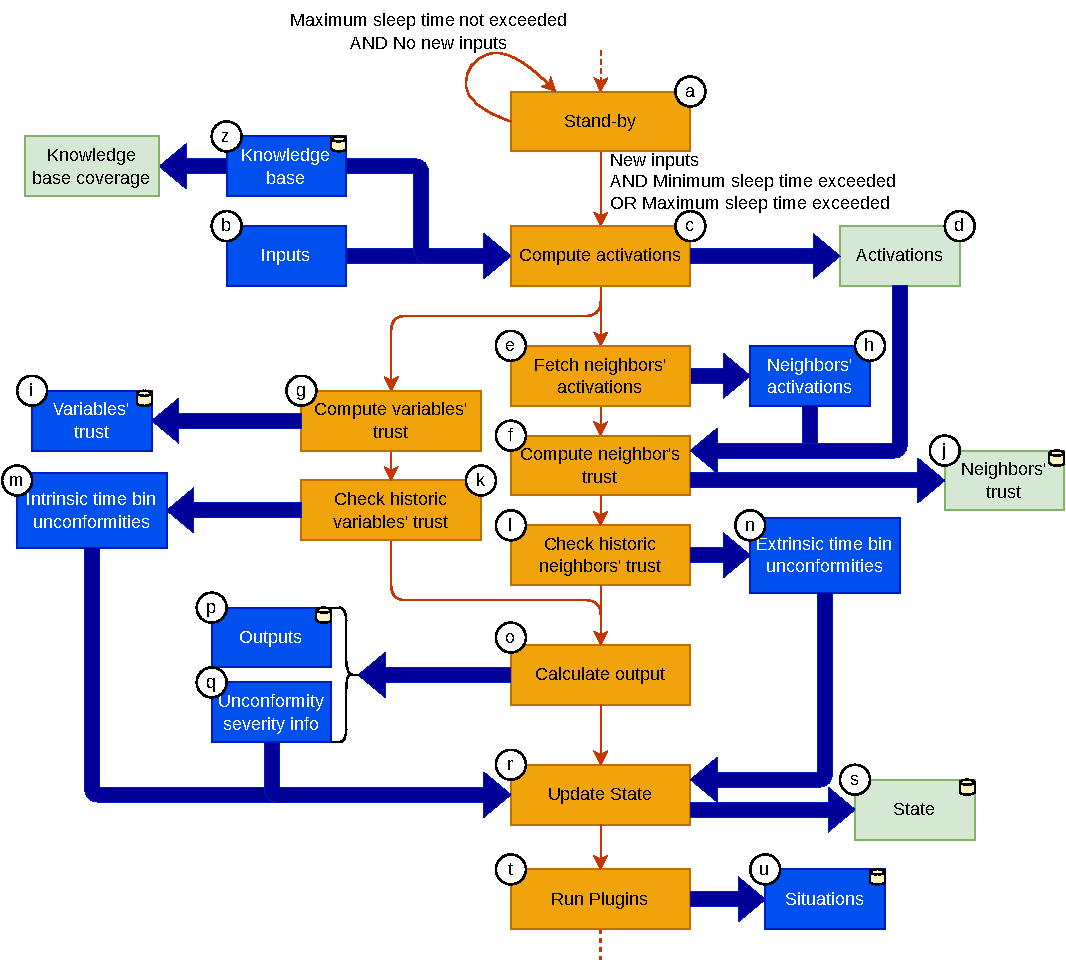
\includegraphics[width=12cm]{figures/chapter4/cell/processes.pdf}
    \caption{Cell's core main loop of processes.}
    \label{fig:cellprocesses}
\end{figure}


In the cell, there are inputs and outputs, which represent the same variables. They are an instantaneous representation of the values that define a cell at a given timestamp, which is continuously rolling. This time instant may be arbitrary and not just the present. Thus, choosing an offset in the future grants it forecasting capabilities.

It features an intrinsic inference process that utilizes the continuous stream of multi-variate time-series data of inputs. Considering all inputs as outputs increase data coherence, which is explored in section \ref{subsec:tempsim}. Then, by modeling uncertainty using a set/interval-based approach, it performs temporal similarity extraction.

\subsection{Temporal similarity extraction} \label{subsec:tempsim}

Temporal similarity extraction the process of identifying recurring patterns in time series data. It involves the identification of past instances where the current state is observed to extract useful information about the system's behavior over time. By identifying historical periods with similar states, temporal similarity extraction can help assess the current state or predict future trends. This technique is common in statistics, for purposes such as estimation and forecasting. Nonetheless, the process of temporal similarity extraction can be challenging due to the complexity and size of time series data, as well as the need to accurately measure and compare similarity across different periods.

Using sets or probability distributions to filter historical data is one approach to simplify the process of temporal similarity extraction in multivariate time series data. This approach assigns membership values to each data point in the time series based on the corresponding set (or distribution) generated from the current cell inputs and eliminates samples past a certain threshold. Representing the cell's variables in a fuzzy or probabilistic manner can better capture the inherent uncertainty in time series data, making the approach relatively robust to noisy or incomplete data. This type of representation is what is stored, for each variable, as the \textbf{inputs}, which can be characterized by:

\begin{itemize}
    \item Classical set: simple uncertainty band (e.g. uncertainty up, down, relative, etc);
    \item Fuzzy number: generalized fuzzy number representation \cite{Zhang2019} (e.g. triangular fuzzy number (a,b,d;h));
    \item Probability distribution: the distribution's characteristics (e.g. mean ($\mu$) and standard deviation ($\delta$) for Gaussian, mean rate of occurence ($\lambda$) for Poisson, etc.);
\end{itemize}

The proposal for similarity extraction in the cell consists of receiving new values for the cell's variables from a data source (sensors or other data acquisition equipment, calculations, forecasting, etc.), generating a classical set, fuzzy number, or probability distribution from the it, and then applying its bounds/membership function or probability density function to the knowledge base (see figure \ref{fig:solo_state_estimation}). The initial choice is to use classical sets since filtering history becomes trivial and efficient: restrict the knowledge base to samples where all variables belong to a corresponding interval.

\paragraph{Self Similarity}

Having a knowledge base and input variables, the cell can perform intrinsic temporal similarity extraction. When filtering historical data with two or more variables, there is a trend of narrowing down the resulting data's space due to the intersection of constraints. The filtered data can then be utilized to construct outputs with equal or less uncertainty, by considering the new bounds of each variable as the bound of the set. This is a straightforward procedure when using classical sets, which can be seen in the following example:

\bigskip

Consider the a cell that is characterized by two variables, which are a function of time: $x(t)$ and $y(t)$. 
From here onwards, on equations refering to a time variable $t$ its defined that present time is equal to $t=0$ and membership functions are represented by $\mu$.
Assume that, at a given instant, these are the new cell inputs:

\begin{equation}
x(0) = 1.0 \rightarrow \mu_{x(0)}(x) =
\begin{cases}
1, & x \in [0.9, 1.1] \\
0, & x \notin [0.9, 1.1] \\
\end{cases}
\end{equation}

\begin{equation}
y(0) = 2.0 \rightarrow \mu_{y(0)}(y) =
\begin{cases}
1, & y \in [1.8, 2.2] \\
0, & y \notin [1.8, 2.2] \\
\end{cases}
\end{equation}

The membership functions $\mu$ are generated considering that $x$ and $y$ are characterized by uniform and symetrical uncertainty, and that the received data ($x(0)$ and $y(0)$) represent its median.

\begin{figure}[h!]
    \centering
    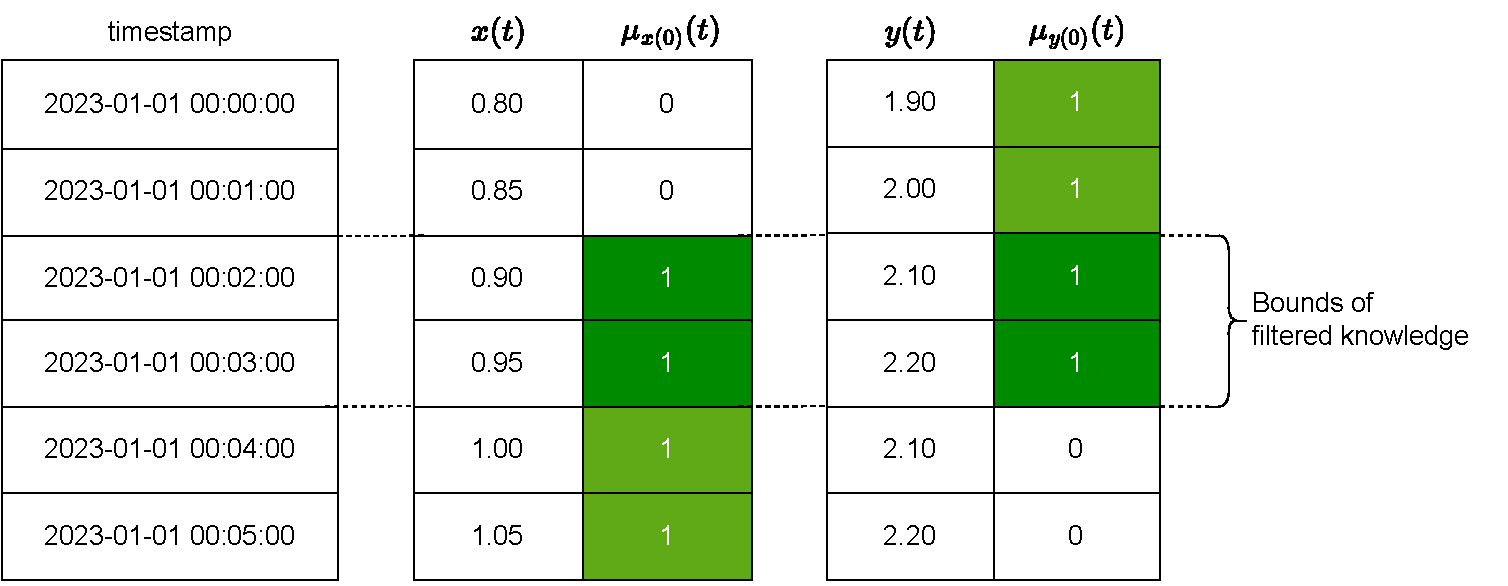
\includegraphics[width=\linewidth]{figures/chapter4/cell/solo_state_estimation.pdf}
    \caption{Visualization of a self similarity extraction example.}
    \label{fig:solo_state_estimation}
\end{figure}


With the knowledge base represented in figure \ref{fig:solo_state_estimation}, the resulting activations will be 2023-01-01 00:02:00 and 2023-01-01 00:03:00. These are the timestamps of past instances where the cell's variables have values belonging to the set generated from new inputs. We can also infer that the values of $x$ and $y$ should reside in a set constrained by the filtered historical values ($x(t)$ and $y(t)$). Therefore, the outputs based on self similarity extraction are:

\begin{equation}
    x'(0) \in [0.90, 0.95]
\end{equation}

\begin{equation}
    y'(0) \in [1.80, 2.20]
\end{equation}

\paragraph{Mutual Similarity}
Capacidade de estimação de estado intrínsica + extrínsica

\subsection{Data model}

O que é publico e privado

\subsection{Connections and Trust}
O que é uma conexão, como se caracteriza, e que valores tem a ela associada

to take advantage of sharing information with neighbours, there comes a need to have trust

\subsection{Events}

TODO


\section{The Hub}

TODO

\section{Implementation}

TODO: escrever sobre a concretização real destas ideias